\section{Subdivision Surfaces}

Subdivision surfaces are a generalization of spline curves / surfaces. They allow for successive refinement and converge to a smooth surface.
\begin{center}
	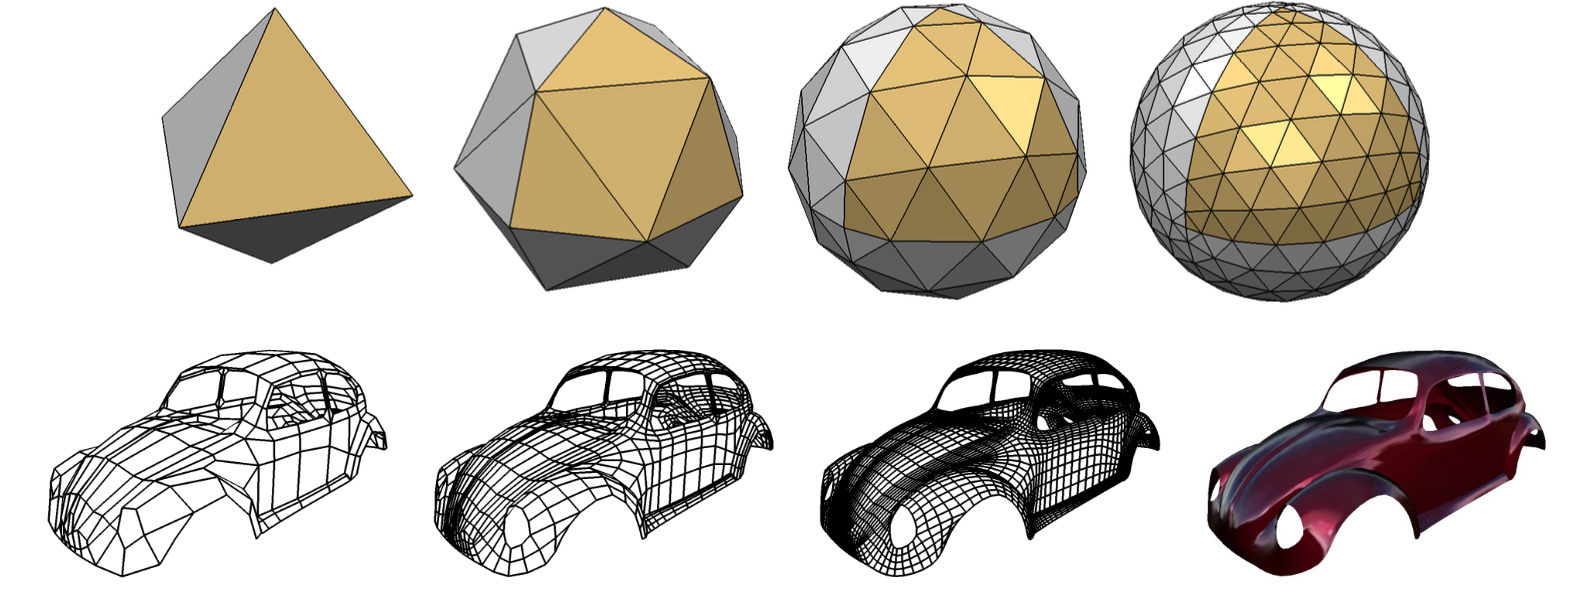
\includegraphics[width=\linewidth]{subdivision.png}
\end{center}

It relies on corner cutting:
\begin{enumerate}
	\item Insert two new vertices at 1/4 and 3/4 of each edge
	\item Remove the old vertices
	\item Connect the new vertices
\end{enumerate}
\begin{center}
	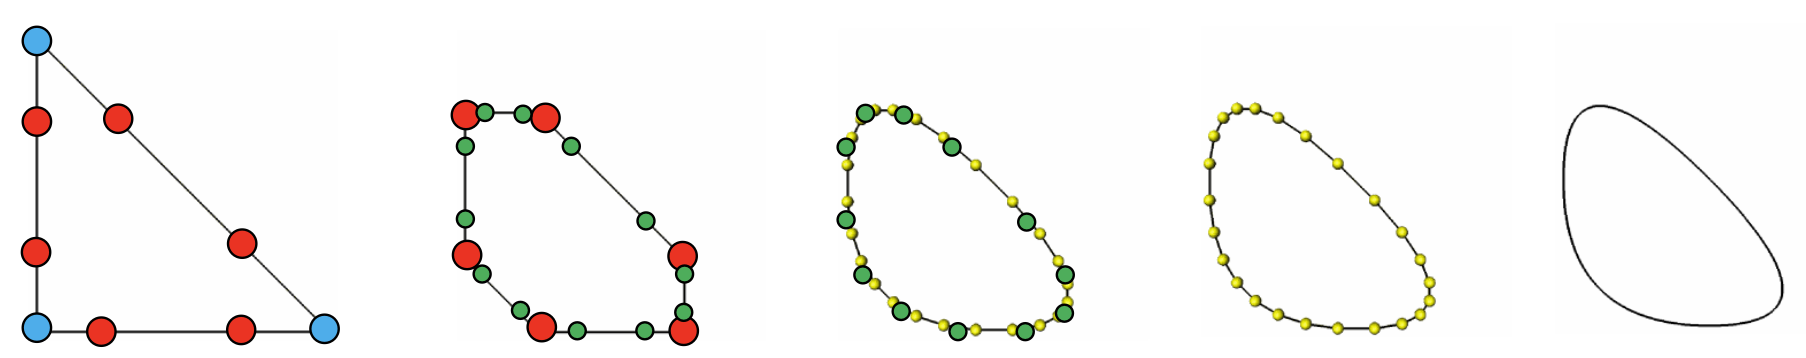
\includegraphics[width=\linewidth]{corner_cutting.png}
\end{center}

There are multiple algorithms for subdivision, with different properties (applied on polygonal mesh or triangle mesh, $G^1$ or $G^2$ continuous etc.). \medskip

One of these algorithms is the \textbf{Loop Subdivision}. It is a generalization of box splines and can be used on triangle meshes. It generates a $G^2$ continuous limit surface:
\begin{center}
	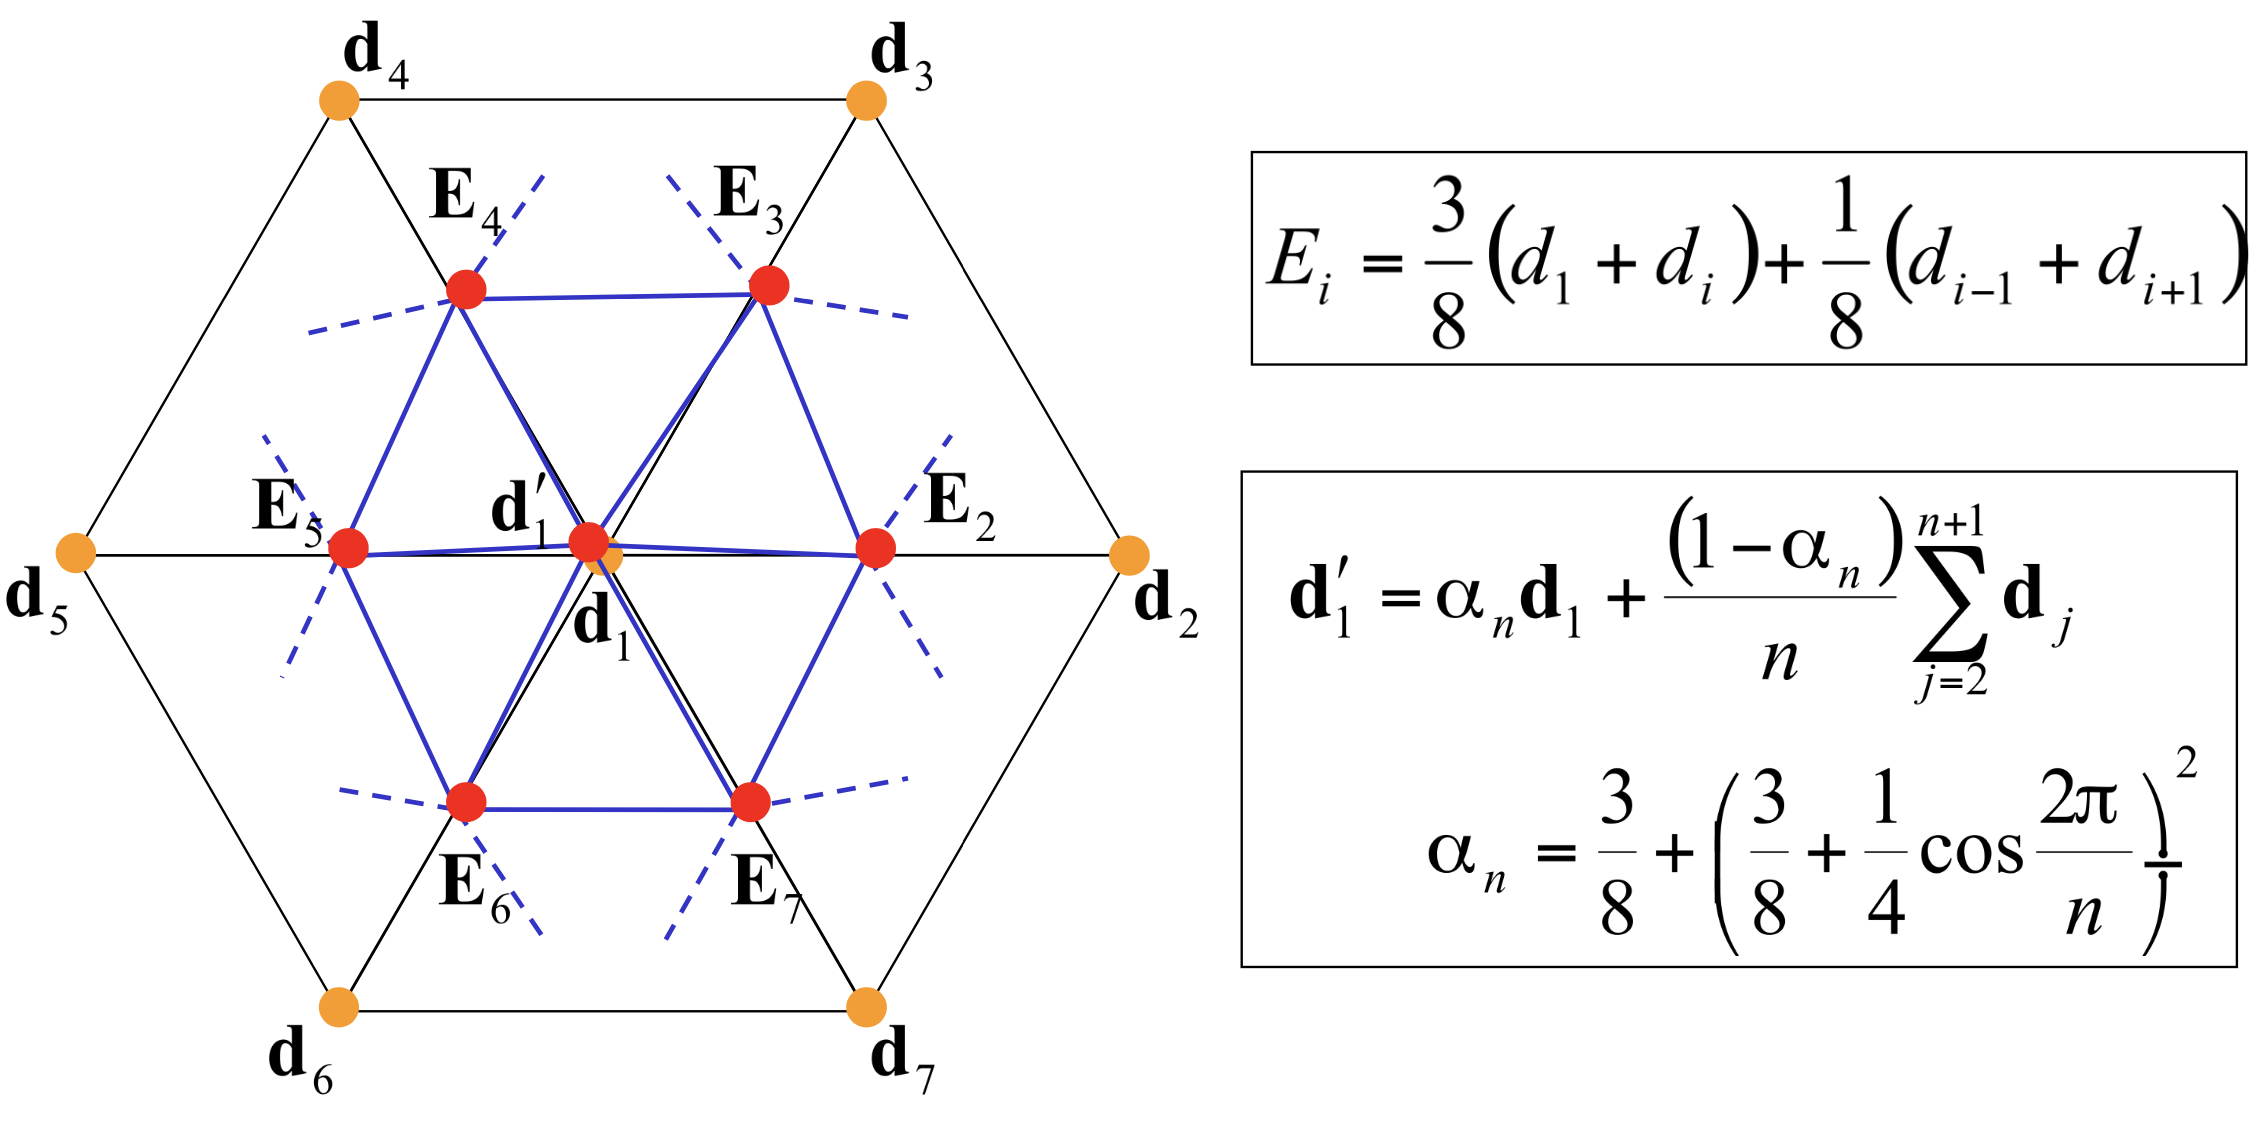
\includegraphics[width=\linewidth]{loop_subdivision.png}
\end{center}
